% coding:utf-8

%FOSAET, a LaTeX-Code for a electrical summary of basic electronics
%Copyright (C) 2013, Daniel Winz, Ervin Mazlagic

%This program is free software; you can redistribute it and/or
%modify it under the terms of the GNU General Public License
%as published by the Free Software Foundation; either version 2
%of the License, or (at your option) any later version.

%This program is distributed in the hope that it will be useful,
%but WITHOUT ANY WARRANTY; without even the implied warranty of
%MERCHANTABILITY or FITNESS FOR A PARTICULAR PURPOSE.  See the
%GNU General Public License for more details.
%----------------------------------------

\subsection{Addierer}
\begin{figure}[h!]
	\centering
	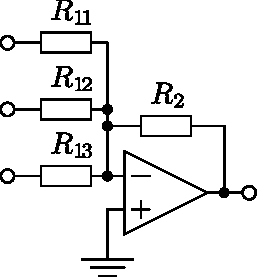
\includegraphics[scale=\schscale]{op_add.pdf}
	\caption{Addierer}
	\label{sch:op-add}
\end{figure}
\[ U_a = - R_2 \cdot \left( \frac{U_{e1}}{R_{11}} + \frac{U_{e2}}{R_{12}} 
+ \frac{U_{e3}}{R_{13}} \right) \]
\[ R_{e1} = R_{11} \qquad R_{e2} = R_{12} \qquad R_{e3} = R_{13} \]
\[ R_a = 0 \]